\documentclass[11pt]{article}

% Geometry roughly matching the AIAA SciTech extended-abstract style.
\usepackage[letterpaper,margin=1in]{geometry}
\usepackage{graphicx}
\usepackage{amsmath,amssymb}
\usepackage[hidelinks]{hyperref}
\usepackage{authblk}
\usepackage{caption}
\usepackage{booktabs}
\usepackage{microtype}
\usepackage{times}

\setlength{\parskip}{4pt}
\setlength{\parindent}{12pt}

\title{\bfseries Two Regimes, One Equation:\\
An Amplification-Factor / Spalart--Allmaras Closure for Transition-Aware RANS}

\author[1,2]{Qiqi Wang\thanks{Associate Professor, Department of Aeronautics and
Astronautics, MIT; AIAA Senior Member.\protect\\
Corresponding author: \texttt{qiqi@flexcompute.com}.}}
\affil[1]{Department of Aeronautics and Astronautics,
Massachusetts Institute of Technology, Cambridge, MA 02139, USA}
\affil[2]{Flexcompute Inc., Watertown, MA 02472, USA}

\date{Submitted to AIAA SciTech Forum 2027, Orlando, FL, January 11--15, 2027 \\
\textit{Technical Discipline: Fluid Dynamics --- Turbulence Modeling /
Boundary-Layer Transition Modeling and Applications}}

\begin{document}

\maketitle

\begin{abstract}
\noindent
Every modern RANS transition closure --- $\gamma$--$Re_\theta$, AFT,
SA-BCM --- adds at least one transport equation to the turbulence model
it accompanies. We show that the extra equation is not needed. The small
range of the Spalart--Allmaras (SA) working variable~$\tilde\nu$, which the
original SA model leaves essentially inert, can be reinterpreted as the
amplification envelope of a Tollmien--Schlichting wave; with one
algebraic modification of the SA source term, a single transport equation
then carries \emph{both} regimes --- an Amplification-Factor-Transport
(AFT) growth law where $\tilde\nu \!\lesssim\! O(\nu)$, and standard SA
turbulent mixing where $\tilde\nu \!\gg\! \nu$. There is no auxiliary
intermittency, no second transported variable, and no extra Jacobian
block in an implicit solver: the entire transition--turbulence problem
is closed by exactly one PDE. A novel
local sensor --- the \emph{Escape Reynolds number} $Re_{\mathrm{esc}}=yv/\nu$
--- is introduced as a robust, integral surrogate for the pressure-gradient
parameter $\lambda_\theta$, letting a single source term span attached
Tollmien--Schlichting amplification, separation-induced (Kelvin--Helmholtz)
breakdown, and fully turbulent eddy-viscosity production. The closure is
plug-compatible with any existing SA-based code, recovers the classical
$e^N$ envelope on a Blasius layer, and retains the standard SA behavior
at fully turbulent conditions. Preliminary 1D and 2D results
calibrate the growth law against $dN/dRe_\theta\!\approx\!0.007$ and reproduce
flat-plate transition trends across freestream turbulence levels. The final
paper will report 2D NACA airfoil predictions of $C_p$, $C_f$, and transition
location compared with XFOIL and the SA-BCM transition family, demonstrating
that a single carefully constructed transport equation can carry both
transition and turbulence physics with accuracy comparable to multi-equation
RANS transition models, while preserving the robustness, low cost, and
implementation simplicity that have made SA ubiquitous in aerospace CFD.
\end{abstract}

\section{Motivation and Purpose}

Transition prediction remains one of the largest sources of uncertainty in
industrial RANS simulation. Most modern transition closures
--- the $\gamma$--$Re_\theta$ model of Langtry \& Menter, the AFT model of
Coder \& Maughmer, and the SA-BCM family of correlation-based variants ---
introduce one or more additional transport equations and a network of
empirical functions to switch between regimes. Each new state variable adds
modeling surface area: tunable coefficients, limiters, and free-stream
ambiguities that must be re-validated for every new geometry. From a software
engineering standpoint each new variable also doubles the burden of
implementation, linearization, and Jacobian-coloring inside an implicit
solver.

By contrast, the original SA model has only one transported quantity, and yet
remains the default closure across much of aerospace CFD. Its near-wall
behavior, free-shear behavior, and zero-time-derivative response in
homogeneous isotropic turbulence are not ``correct'' in any detailed sense,
but they are robust, predictable, and easy to debug in flows the model's
authors never anticipated. There is a parsimony in this design that has
proven remarkably durable.

\textbf{The objective of this paper is to show that the same parsimony can be
extended to laminar-to-turbulent transition.} Rather than carry a separate
amplification factor or intermittency, we reinterpret the small-$\tilde\nu$
range of the SA equation --- the regime in which the standard model
contributes negligibly to the eddy viscosity --- as the natural state space
for a Tollmien--Schlichting (TS) envelope. The AFT physics is folded into the
production and destruction terms of the SA equation itself, and the closure
recovers each individual model in its respective limit.

\section{Technical Foundation}

\subsection{One transport equation, two regimes}

The model retains the SA conservation form,
\begin{equation}
\frac{D\tilde\nu}{Dt} \;=\; P(\tilde\nu, \nabla u, d) \;-\; D(\tilde\nu, d)
\;+\; T(\tilde\nu, \nabla u) \;+\; \frac{1}{\sigma}\nabla\!\cdot\!\big[(\nu+\tilde\nu)\nabla\tilde\nu\big]
\;+\; \frac{c_{b2}}{\sigma}|\nabla\tilde\nu|^2,
\label{eq:onevar}
\end{equation}
in which the diffusion, near-wall destruction, and gradient-energy structure
are inherited from the original Spalart--Allmaras formulation. The novelty
sits in the transition-active production term~$T$, designed so that
\eqref{eq:onevar} reduces to standard SA whenever $\tilde\nu$ is large
relative to the molecular viscosity, and to an AFT amplification equation
whenever $\tilde\nu$ is small.

\subsection{A local replacement for $Re_\theta$}

In the classical $e^N$ method, the log-amplitude of the most unstable TS wave
grows almost linearly with the momentum-thickness Reynolds number,
$dN/dRe_\theta\!\approx\!0.007$ for a Blasius layer. Adopting this rule
inside a RANS code is awkward because $Re_\theta$ is non-local: it requires
integrating the velocity profile from the wall to a boundary-layer edge that
may not be cleanly defined in 2D/3D RANS fields. We instead use the
\emph{vorticity Reynolds number}
\begin{equation}
Re_\Omega(x,y) \;=\; \frac{y^2|\Omega|}{\nu},
\end{equation}
which is built from purely local quantities and tracks $Re_\theta$
remarkably closely in attached, two-dimensional boundary layers; the peak of
$Re_\Omega$ remains within a few percent of $2.2\,Re_\theta$ across the entire
unstable Blasius range. This local proxy is the basis of the production term:
\begin{equation}
T(\tilde\nu,\nabla u) \;=\; f_\lambda\!\big(Re_{\mathrm{esc}}, Re_\Omega\big)\,\Omega\,\tilde\nu,
\qquad
f_\lambda \;=\; \frac{0.007\,\max(0,\,Re_\Omega - 400)}{400 + 0.035\,(Re_\Omega - 400)}.
\label{eq:flam-blasius}
\end{equation}
The constant $0.007$ is fixed analytically by requiring~\eqref{eq:flam-blasius}
to reproduce the canonical $e^N$ envelope rate when integrated through the
wall-normal direction of a Blasius profile (Fig.~\ref{fig:blasius-growth},
right panel).

\subsection{An integral pressure-gradient sensor: $Re_{\mathrm{esc}}$}

Real boundary layers are not Blasius. The $e^N$ envelope rate
$dN/dRe_\theta$ varies by an order of magnitude with shape factor:
favorable gradients suppress amplification, adverse gradients accelerate it,
and approaching separation triggers the Kelvin--Helmholtz mechanism. Existing
local closures (Langtry--Menter, Coder--Maughmer) sense this through
$\lambda_\theta\!\propto\!\partial v/\partial y$, which is brittle because $v$
is small and its derivative is sensitive to mass-imbalance noise. We instead
introduce
\begin{equation}
Re_{\mathrm{esc}} \;\equiv\; \frac{d}{\nu}\frac{Dd}{Dt} \;\approx\; \frac{y\,v}{\nu},
\label{eq:Reesc}
\end{equation}
the \emph{Escape Reynolds number}: the wall-normal integral of the same
quantity $\partial v/\partial y$ that traditional sensors differentiate.
Dimensional analysis on Falkner--Skan similarity solutions confirms that
$Re_{\mathrm{esc}}$ is independent of $Re_x$ and depends primarily on the
Hartree parameter~$\beta$ --- it is small in stagnation flow, $\sim\!2$ in
Blasius flow, and grows past 4 as separation approaches. Its integral
character makes it numerically smooth in unstructured RANS fields where the
direct derivative is noisy.

We then close~\eqref{eq:flam-blasius} into a 2D map
$f_\lambda(Re_{\mathrm{esc}},Re_\Omega)$ with three asymptotic branches:
(i) the viscous TS envelope ($1.4\!<\!Re_{\mathrm{esc}}\!<\!3$), targeting
$\lambda\approx 0.0025$; (ii) the inviscid shear limit
($Re_{\mathrm{esc}}\!>\!20$ or $Re_\Omega\!\gg\!10^4$), targeting Michalke's
hyperbolic-tangent maximum $\lambda_{\max}\approx 0.19$; and
(iii) a linear blend in between. A simple gate $Re_\Omega\!>\!100$ keeps
the production term dormant in irrotational regions of the freestream.

\section{Preliminary Results}

\subsection{Calibration on a Blasius boundary layer}

\begin{figure}[t]
\centering
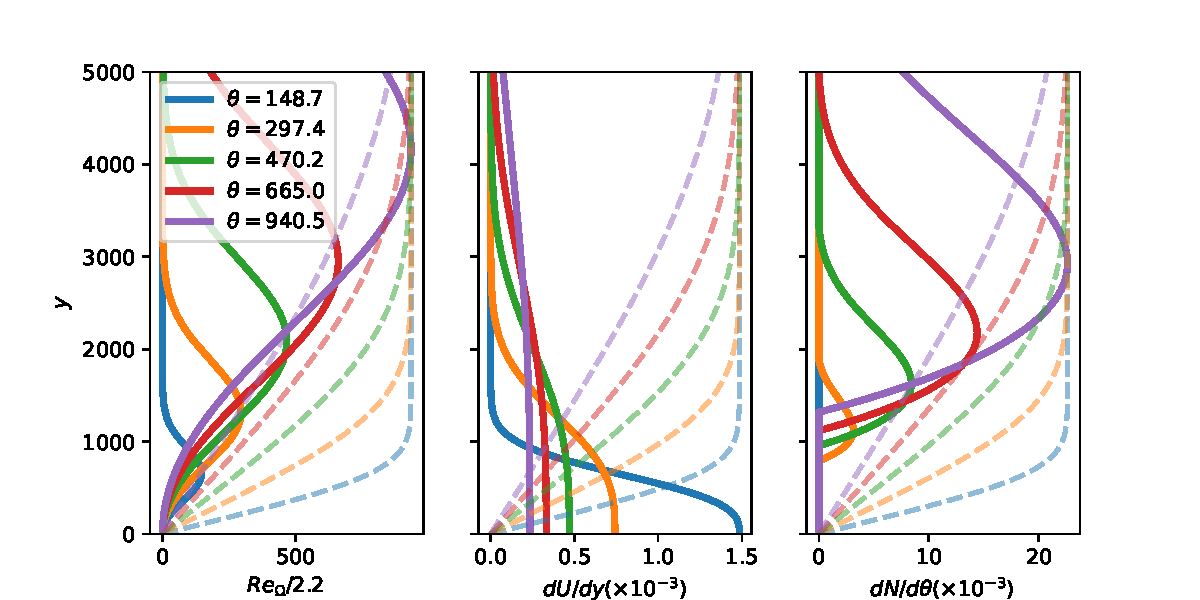
\includegraphics[width=0.95\textwidth]{fig/blasius_ReOmega_growth.pdf}
\caption{Calibration of $Re_\Omega$-based growth in a Blasius layer.
\textit{Left:} streamwise profiles of $u$ (solid) and $Re_\Omega$ (dashed);
the peak of $Re_\Omega$ tracks $2.2\,Re_\theta$. \textit{Middle:} mean shear
$\partial u/\partial y$ entering~\eqref{eq:flam-blasius}.
\textit{Right:} effective $dN/dRe_\theta$ from the local production
integrated wall-normally; the model recovers the textbook $e^N$ growth
rate of $0.007$ once $Re_\Omega^{\max}\!\gtrsim\!1200$.}
\label{fig:blasius-growth}
\end{figure}

Figure~\ref{fig:blasius-growth} shows that the calibration of
\eqref{eq:flam-blasius} reproduces the classical envelope rate exactly. A
finite-volume integration of the full transport equation, using
$\hat\nu(x\!=\!0,y)\equiv 1$ as the inlet, then yields the $N$-factor field
of Fig.~\ref{fig:blasius-nuhat}: contours of $N=\ln\hat\nu$ remain confined
to the TS-active band between $\theta$ and $\delta_{99}$ and grow many
$e$-folds before cross-stream diffusion can homogenize the envelope, in
quantitative agreement with $e^N$ predictions. This confirms the design
principle that the local production term, not the diffusion, sets the
transition location.

\begin{figure}[t]
\centering
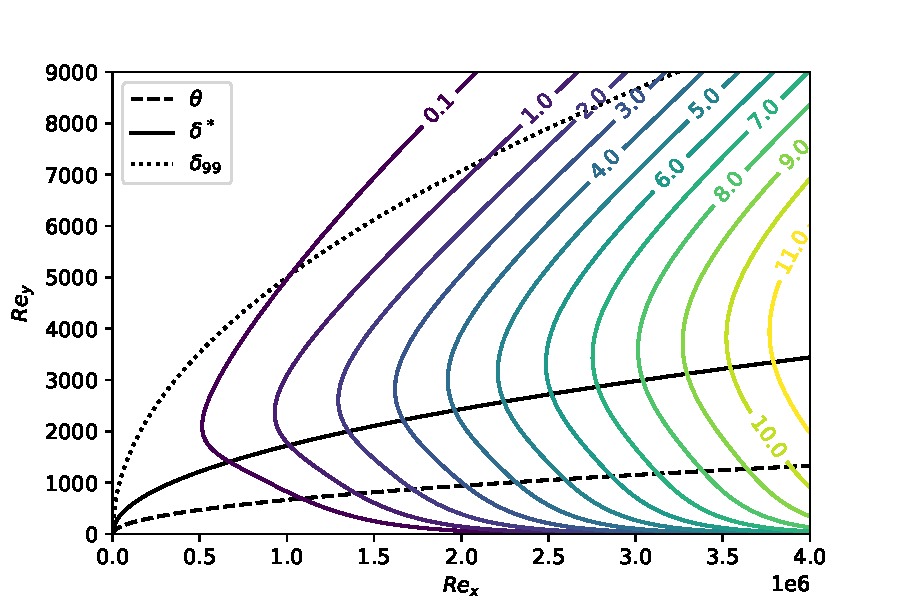
\includegraphics[width=0.7\textwidth]{fig/blasius_nuHat_solution.pdf}
\caption{Solution of the full transport equation for $\hat\nu$ in a Blasius
layer with uniform inlet $\hat\nu(0,y)\!=\!1$. Contours of $N=\ln\hat\nu$
(0.1--11) remain confined to the TS band marked by $\theta$, $\delta^*$,
and $\delta_{99}$, demonstrating that local production --- not diffusion ---
drives the streamwise march of transition.}
\label{fig:blasius-nuhat}
\end{figure}

\subsection{Flat-plate parameter sweeps}

\begin{figure}[t]
\centering
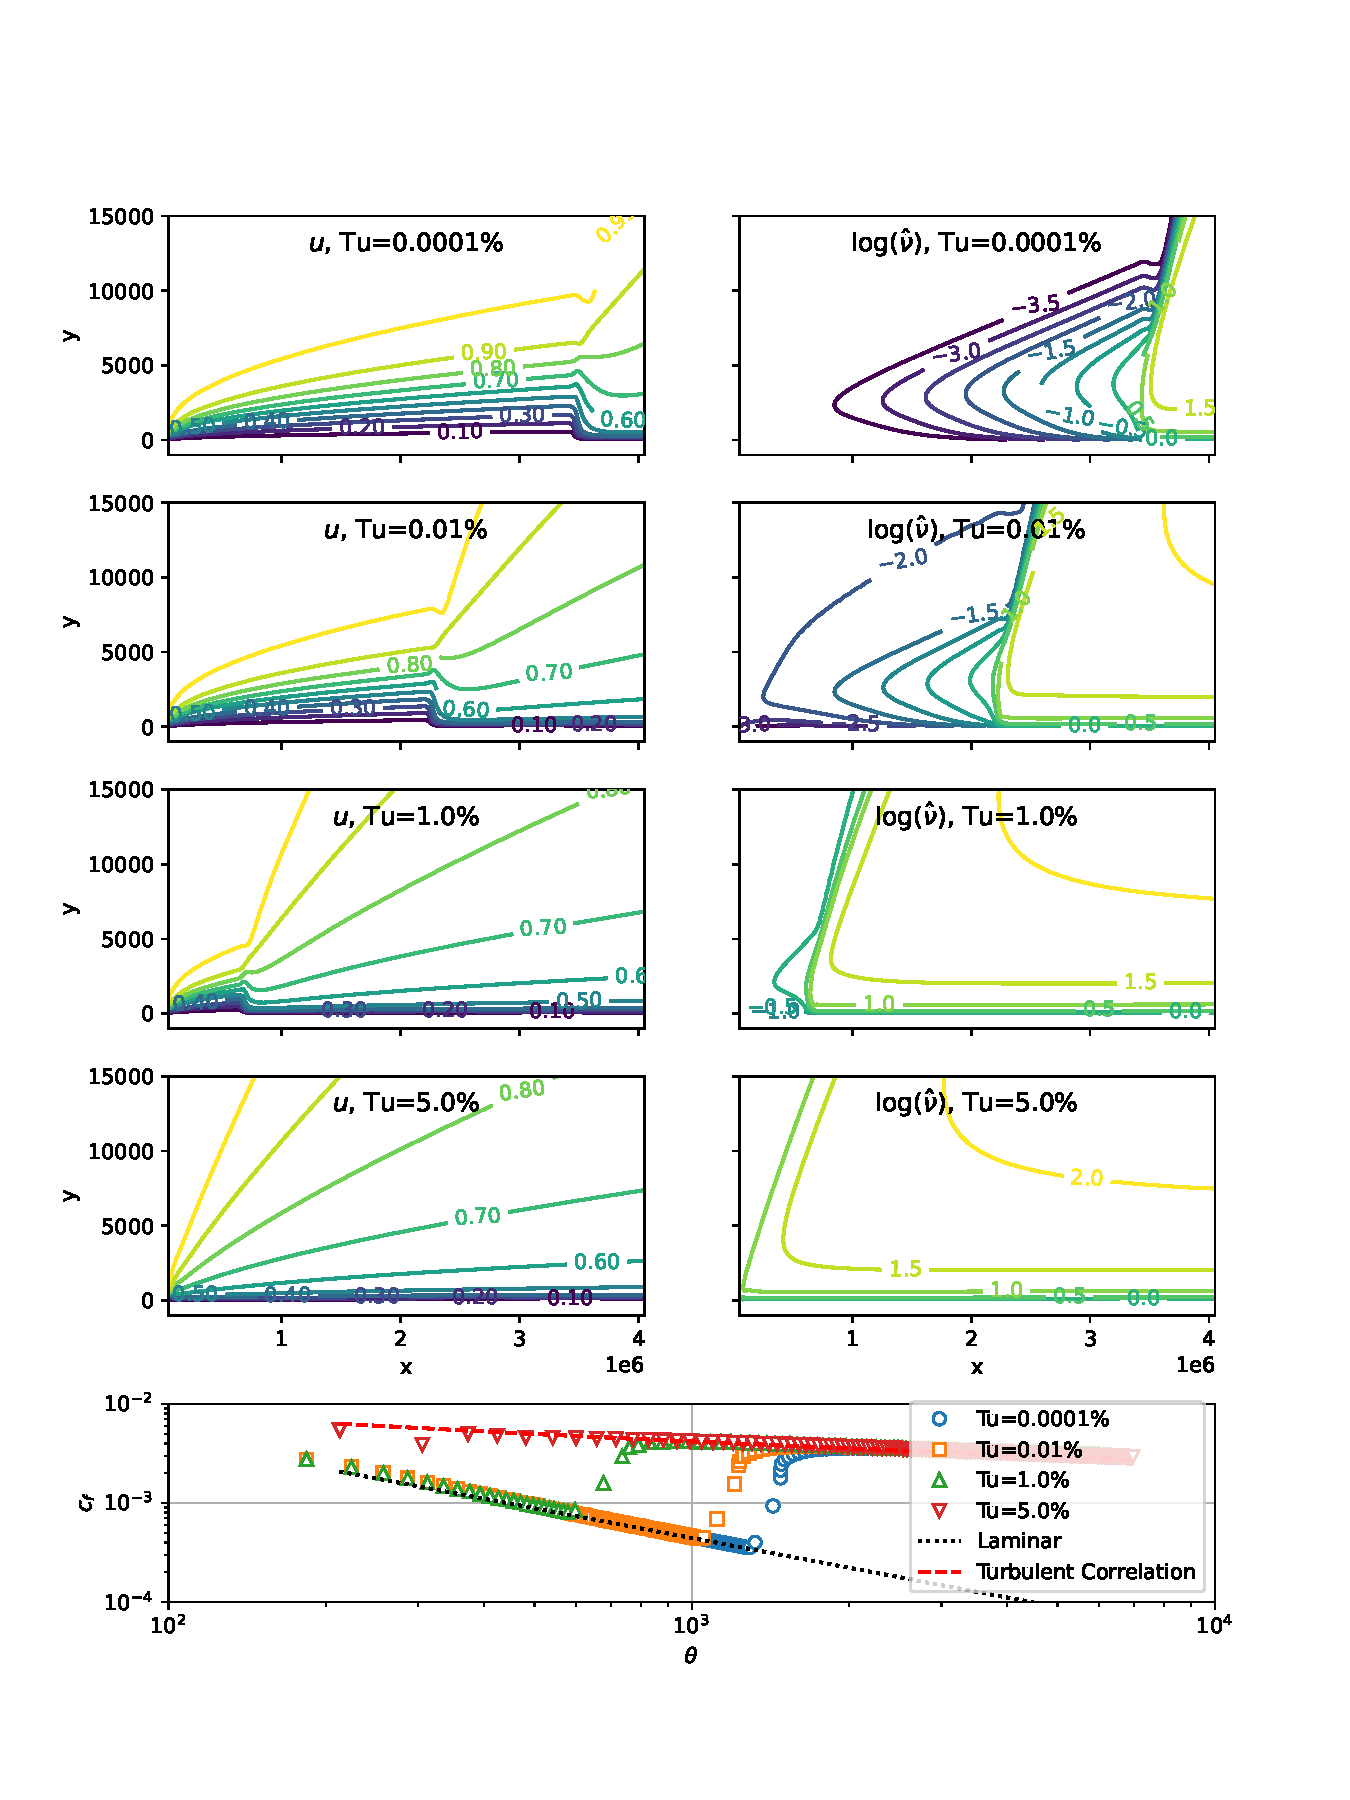
\includegraphics[width=0.95\textwidth]{fig/flat_plate_batch.pdf}
\caption{Flat-plate transition predictions across a range of inlet
amplitudes (analogous to freestream turbulence levels). Skin friction (top)
and shape factor (bottom) trace the canonical laminar-to-turbulent
transition path; transition $Re_x$ shifts upstream with disturbance amplitude
in agreement with the Mack--$N_\mathrm{crit}$ trend.}
\label{fig:flat-plate-batch}
\end{figure}

A coupled boundary-layer/AFT--SA solver in the companion code base
(\texttt{src/solvers/boundary\_layer\_solvers.py}) was used to sweep the
inlet disturbance amplitude (a stand-in for freestream turbulence intensity)
and verify the transition-onset trend. Figure~\ref{fig:flat-plate-batch}
shows the resulting $C_f(Re_x)$ and $H(Re_x)$ envelopes; the model produces
the qualitatively correct Mack--$N_\mathrm{crit}$ shift of transition
location with disturbance amplitude.

\subsection{2D RANS implementation}

The closure is implemented in a JAX-accelerated 2D structured-grid RANS
solver based on the Artificial Compressibility Method, JST convective fluxes,
and a 5-stage Runge--Kutta time integrator. The solver shares its discrete
operators between the SA branch and the AFT branch; switching between the
two costs only an additional algebraic evaluation of $f_\lambda$ inside the
existing \texttt{compute\_sa\_source\_jax} kernel. The end-to-end NACA~0012
case at $Re=1\!\times\!10^6$, $\alpha=0^\circ$ has been brought to converged
solution and is being used for the validation campaign described below.

\section{Expected Final Results}

The final SciTech paper will deliver three categories of validation:

\begin{enumerate}\setlength{\itemsep}{2pt}
\item \textbf{Canonical flat plate.} Schubauer--Klebanoff and ERCOFTAC-T3
test cases at multiple turbulence intensities and pressure gradients,
comparing transition location and skin-friction recovery against
experiments and the SA-BCM and Langtry--Menter $\gamma$--$Re_\theta$ models.
\item \textbf{2D airfoils.} NACA~0012 and NLF~0416 over an angle-of-attack
sweep at $Re=10^6$--$9\!\times\!10^6$, comparing $C_p$, $C_f$, transition
location, and integrated $C_l$, $C_d$ against XFOIL (the reference
$e^N$-based prediction at low freestream disturbance) and against
correlation-based RANS transition models.
\item \textbf{Robustness in off-design conditions.} Cases with mild
trailing-edge separation and laminar separation bubbles, where
correlation-based models are known to be brittle; the goal is to demonstrate
that the $Re_{\mathrm{esc}}$-based switch into the inviscid (KH) branch
prevents unphysical persistence of laminar separation, without requiring
case-by-case retuning.
\end{enumerate}

\section{Significance for Aerospace CFD}

If successful, the AFT--SA closure will collapse what is currently a
two- or three-equation transition modeling problem onto a single transport
equation that is structurally identical to SA. For aerospace solvers that
already linearize SA implicitly (e.g.\ in JFNK or Newton--Krylov frameworks),
adoption requires only an algebraic modification of the source term --- no
new conservation variables, no new boundary conditions, no new Jacobian
blocks. This has the potential to make modern transition prediction
accessible to industrial design workflows that currently default to fully
turbulent SA out of implementation cost, while preserving the robustness
that has made SA the workhorse closure of aerospace CFD for three decades.

\section*{Acknowledgments}
The author thanks Philippe Spalart and Mark Drela for insightful discussions
that helped shape the ideas in this work. Computational resources were
provided by Flexcompute Inc. The code and reproduction scripts are openly
released at \url{https://github.com/qiqi/aft-sa}.

\section*{Selected References}
\small
\begin{enumerate}\setlength{\itemsep}{0pt}
\item Spalart, P.\,R., and Allmaras, S.\,R., ``A One-Equation Turbulence Model
for Aerodynamic Flows,'' \textit{La Recherche A\'{e}rospatiale}, No.~1, 1994.
\item Coder, J.\,G., and Maughmer, M.\,D., ``Computational Fluid Dynamics
Compatible Transition Modeling Using an Amplification Factor Transport
Equation,'' \textit{AIAA Journal}, Vol.~52, No.~11, 2014.
\item Langtry, R.\,B., and Menter, F.\,R., ``Correlation-Based Transition
Modeling for Unstructured Parallelized Computational Fluid Dynamics Codes,''
\textit{AIAA Journal}, Vol.~47, No.~12, 2009.
\item Drela, M., and Giles, M.\,B., ``Viscous-Inviscid Analysis of Transonic
and Low Reynolds Number Airfoils,'' \textit{AIAA Journal}, Vol.~25, No.~10,
1987.
\item van Ingen, J.\,L., ``The $e^N$ Method for Transition Prediction:
Historical Review of Work at TU Delft,'' AIAA Paper 2008-3830, 2008.
\item Mura, S., and \c{C}akmak\c{c}{\i}o\u{g}lu, S.\,C., ``A Revised
One-Equation Transitional Model for External Aerodynamics,'' AIAA Paper
2020-2735, 2020.
\item Michalke, A., ``On the Inviscid Instability of the Hyperbolic-Tangent
Velocity Profile,'' \textit{Journal of Fluid Mechanics}, Vol.~19, 1964.
\item van Driest, E.\,R., and Blumer, C.\,B., ``Boundary Layer Transition:
Free-Stream Turbulence and Pressure Gradient Effects,'' \textit{AIAA Journal},
Vol.~1, No.~6, 1963.
\end{enumerate}

\end{document}
